\chapter{Additional informations on computation}
\label{appendix:add_info}
\section*{Element-wise product}
The element-wise product between two matrix $\mathbf{A}$ and $\mathbf{B}$ is noted $\mathbf{A} \odot \mathbf{B}$ and is defined in the following way:\\
For two matrices $\mathbf{A}$, $\mathbf{B}$ of same dimensions $n \times m$, the element-wise product is a $n \times m$ matrix where the elements are defined by:
\[(\mathbf{A} \odot \mathbf{B})_{i,j} = (\mathbf{A})_{i,j} \cdot (\mathbf{B})_{i,j}\]
The product is undefined for matrices of different dimensions

\section*{Kronecker product}
The Kronecker product of two matrix $\mathbf{A}$ and $\mathbf{B}$ of respective dimensions $n \times m$ and $p \times q$ is a $np \times mq$ block matrix where the elements are defined by:
\[\mathbf { A } \otimes \mathbf { B } = 
\left[ 
\begin{array}
 { c c c } { a _ { 11 } \mathbf { B } } & { \cdots } & { a _ { 1 n } \mathbf { B } } \\ { \vdots } & { \ddots } & { \vdots } \\ { a _ { m 1 } \mathbf { B } } & { \cdots } & { a _ { m n } \mathbf { B } } 
\end{array} 
\right]\] 

\section*{Polynomials splines}
\textcite{fahrmeir_regression:_2013} state that a function $f : [ a , b ] \rightarrow \mathbb { R }$ is called a polynomial spline of degree $l \geq 0$ with knots $a = \kappa _ { 1 } < \ldots < \kappa _ { m } = b$, if it fulfills the following conditions:
\begin{enumerate}
\item $f(z)$ is $(l-1)$ times continuously differentiable. The special case of $l = 1$ corresponds to $f(z)$ being continuous (but not differentiable). We do not state any smoothness requirements for $f(z)$ when $l=0$.
\item $f(z)$ is a polynomial of degree $l$ on intervals $\left[ \kappa _ { j } , \kappa _ { j + 1 } \right)$ defined by the knots.
\end{enumerate}
Moreover, it can be shown that each polynomial spline of degree $l$ with
knots $\kappa _ { 1 } < \ldots < \kappa _ { m }$ can be uniquely determined as a linear combination of the $d = l+m-1$ functions
$B_1, \dots , B_d$, called the \textit{basis functions}, since we can uniquely represent all polynomials splines by using these functions.

\subsection*{B-splines}
B-splines are polynomial splines with specific basis functions. B-spline basis functions are constructed
from piecewise polynomials that are fused smoothly at the knots to achieve the desired smoothness constraints. More specifically, a B-spline basis function consists
of $(l+1)$ polynomial pieces of degree $l$ , which are joined in an $(l-1)$ continuously differentiable way. All B-spline basis functions are set up based on a given knot configuration. Using the complete basis, the function $f(z)$ can again be represented through a linear combination of $d = m + l-1$ basis
functions, i.e.,
\[f ( z ) = \sum _ { j = 1 } ^ { d } \gamma _ { j } B _ { j } ( z )\text{.}\]
The B-splines of order $l=0$ can be written as
\[B _ { j } ^ { 0 } ( z ) = \left\{ \begin{array} { l l } { 1 } & { \kappa _ { j } \leq z < \kappa _ { j + 1 } } \\ { 0 } & { \text { otherwise } } \end{array} \right. \quad j = 1 , \ldots , d - 1\]
and the B-splines for higher order $l$ can be written as
\[B _ { j } ^ { l } ( z ) = \frac { z - \kappa _ { j - l } } { \kappa _ { j } - \kappa _ { j - l } } B _ { j - 1 } ^ { l - 1 } ( z ) + \frac { \kappa _ { j + 1 } - z } { \kappa _ { j + 1 } - \kappa _ { j + 1 - l } } B _ { j } ^ { l - 1 } ( z ) \text{.}\]
The estimation of a polynomial spline in B-spline representation can be traced back to the estimation of a linear model with a large number of parameters and design matrix 
\[\mathbf{Z}= \left( \begin{array} { c c c } { B _ { 1 } ^ { l } \left( z _ { 1 } \right) } & { \dots } & { B _ { d } ^ { l } \left( z _ { 1 } \right) } \\ { \vdots } & { } & { \vdots } \\ { B _ { 1 } ^ { l } \left( z _ { n } \right) } & { \dots } & { B _ { d } ^ { l } \left( z _ { n } \right) } \end{array} \right) \text{.} \]
The linear combination of basis functions can then be written in matrix form
\[ \mathbf{y} = \mathbf{Z} \mbox{\boldmath$\gamma$} \]
where the coefficient matrix, {\boldmath$\gamma$} can be estimated using least squares.\\
The estimation of a B-spline fit can be summarized in three steps:
\begin{enumerate}
\item We calculate a complete B-spline basis for a given number of knots.
\item The least squares estimate {\boldmath$\hat{\gamma}$} yields an amplitude $\hat{\gamma_j}$ for the scaling of every basis function.
\item We obtain the final estimate by summing the scaled basis function.
\end{enumerate}

\subsection*{Penalized splines}
We clearly see that the quality of the estimation by polynomials splines highly depends on the number of knots and that this can easily lead to an over-fitting issue. To overcome this problem, \textit{penalized splines (P-splines)} introduce a roughness penalty term that prevents over-fitting and minimize a \textit{penalized least squares (PLS) criterion} instead of the usual least squares criterion.\\
To characterize the smoothness of any type of function, the
use of (squared) derivatives is appropriate, since these represent measures for the variability of a function. Therefore penalties based on the second derivative, such as
\[ \lambda \int \left( f ^ { \prime \prime } ( z ) \right) ^ { 2 } d z\text{,} \]
are particularly attractive since they measure the curvature of a function. Since we know that the first derivative of a B-spline can be written as a function of the first differences of the corresponding coefficient vector, we can use differences of a higher order $r$ if we aim at a smooth function in terms of $r$th-order derivatives. This leads to the penalized residual sum of squares
\[\operatorname { PLS } ( \lambda ) = \sum _ { i = 1 } ^ { n } \left( y _ { i } - \sum _ { j = 1 } ^ { d } \gamma _ { j } B _ { j } \left( z _ { i } \right) \right) ^ { 2 } + \lambda \sum _ { j = r + 1 } ^ { d } \left( \Delta ^ { r } \gamma _ { j } \right) ^ { 2 }\text{,}\]
where $\Delta^r$ denotes the $r$th-order differences.The smoothing parameter $\lambda \geq 0$ controls the compromise between fidelity to the data and smoothness of the resulting function estimate. The PLS criterion can be rewritten using matrix notation
\[ \operatorname { PLS } ( \lambda ) = ( \mathbf{y} - \mathbf{Z} \boldsymbol{\gamma} ) ^ { \prime } (  \mathbf{y} - \mathbf{Z} \boldsymbol{\gamma}) + \lambda \boldsymbol{\gamma} ^ { \prime }\mathbf{K_r} \boldsymbol{\gamma} \]
where $\mathbf{K_r}$ is the $r$th-order difference penalty matrix, and can be decomposed as $\mathbf{D_r}\prime \mathbf{D_r}$ with $D_r$ the $r$th-order difference matrix.
The smoothing parameter $\lambda \geq 0$ controls the compromise between fidelity to the data and smoothness of the resulting function estimate. The PLS estimate of the coefficient matrix is then 
\[ \hat { \boldsymbol{\gamma} } = \left(\mathbf{ Z} ^ { \prime } \mathbf {Z} + \lambda \mathbf{K} \right) ^ { - 1 }\mathbf{ Z} ^ { \prime }\mathbf{ y} \text{.}\]
For more detailed information about polynomials splines, please refer to \textcite{fahrmeir_regression:_2013} and \textcite{eilers_flexible_1996}

\clearpage

\chapter{Hoagland solution}
\label{appendix:hoagland}

\rowcolors{2}{gray!25}{white}

\begin{table}[hbtp]
    \centering
    \caption{Composition of the \textit{Hoagland} nutritive solution. The pH must be adjusted to 5.0 using \ch{HCl} 1\% before using.}
    \label{tab:my_label}
    \begin{threeparttable}
    \begin{tabular}{>{\bfseries}p{4cm} p{4cm} p{4cm}}
    \toprule
        Components & \textbf{Concentration (g/L)} & \textbf{ml for 25L of solution}\tnote{1} \\
    \midrule
        2M \ch{KNO3} & 202 & 62.5 \\
        2M \ch{Ca(NO3)2} x \ch{4 H2O}  & 472 & 62.5\\
        2M \ch{MgSO4} x \ch{7 H2O} & 493 & 25\\
        1M \ch{NH4NO3} & 80 & 25\\
        Minors: \newline
        \ch{H3BO3} \newline
        \ch{MnCl2} x \ch{4 H2O} \newline
        \ch{ZnSO4} x \ch{7 H2O} \newline
        \ch{CuSO4} \newline
        \ch{H3MoO4} x \ch{H2O} or \newline
        \ch{Na2MoO4} x \ch{2 H2O} & 
        ~    \newline
        2.86 \newline
        1.81 \newline
        0.22 \newline
        0.051 \newline
        0.09 \newline 
        0.12 & 
        ~    \newline
        ~    \newline
        ~    \newline
        25 \tnote{2} \\
        1M \ch{KH2PO4} (ph to 6.0 with 3M \ch{KOH}) & 136 & 12.5\\
        Iron (Sprint 138 iron chelate) & 15 & 75\\
    \bottomrule
    \end{tabular}
    \begin{tablenotes}\footnotesize
        \item[1] For a 1:1 solution to use with 25L of water.
        \item[2] All the minors elements are grouped, in the right proportions, in a "minor" solution.
    \end{tablenotes}
    \end{threeparttable}
\end{table}

\chapter{Phenotyping platform information file}
\label{appendix:platform_info}
\clearpage
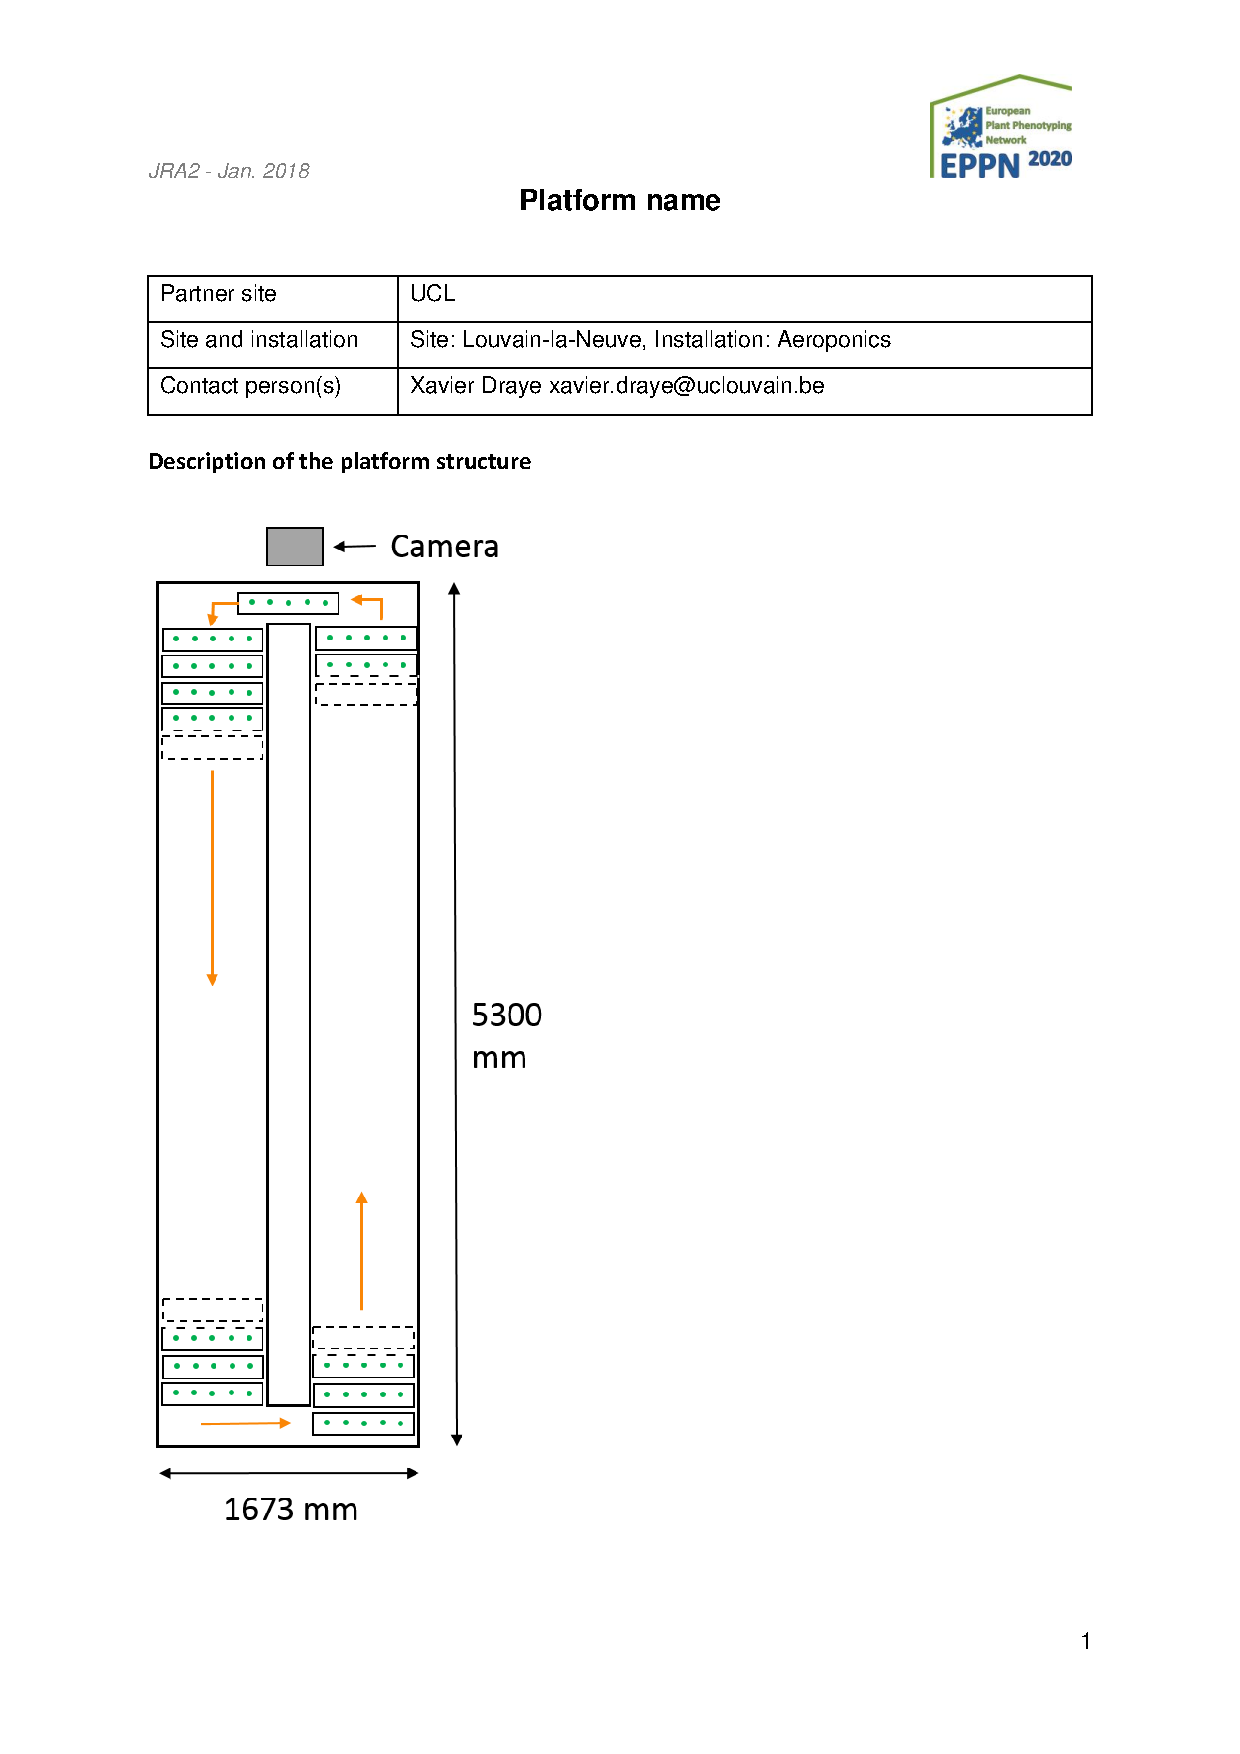
\includepdf[pages=-,pagecommand={},width=\textwidth]{extra/platform_info.pdf}
